%% BioMed_Central_Tex_Template_v1.06
%%                                      %
%  bmc_article.tex            ver: 1.06 %
%                                       %

%%IMPORTANT: do not delete the first line of this template
%%It must be present to enable the BMC Submission system to
%%recognise this template!!

%%%%%%%%%%%%%%%%%%%%%%%%%%%%%%%%%%%%%%%%%
%%                                     %%
%%  LaTeX template for BioMed Central  %%
%%     journal article submissions     %%
%%                                     %%
%%          <8 June 2012>              %%
%%                                     %%
%%                                     %%
%%%%%%%%%%%%%%%%%%%%%%%%%%%%%%%%%%%%%%%%%


%%%%%%%%%%%%%%%%%%%%%%%%%%%%%%%%%%%%%%%%%%%%%%%%%%%%%%%%%%%%%%%%%%%%%
%%                                                                 %%
%% For instructions on how to fill out this Tex template           %%
%% document please refer to Readme.html and the instructions for   %%
%% authors page on the biomed central website                      %%
%% http://www.biomedcentral.com/info/authors/                      %%
%%                                                                 %%
%% Please do not use \input{...} to include other tex files.       %%
%% Submit your LaTeX manuscript as one .tex document.              %%
%%                                                                 %%
%% All additional figures and files should be attached             %%
%% separately and not embedded in the \TeX\ document itself.       %%
%%                                                                 %%
%% BioMed Central currently use the MikTex distribution of         %%
%% TeX for Windows) of TeX and LaTeX.  This is available from      %%
%% http://www.miktex.org                                           %%
%%                                                                 %%
%%%%%%%%%%%%%%%%%%%%%%%%%%%%%%%%%%%%%%%%%%%%%%%%%%%%%%%%%%%%%%%%%%%%%

%%% additional documentclass options:
%  [doublespacing]
%  [linenumbers]   - put the line numbers on margins

%%% loading packages, author definitions

\documentclass[twocolumn]{bmcart}% uncomment this for twocolumn layout and comment line below
%\documentclass{bmcart}

%%% Load packages
%\usepackage{amsthm,amsmath}
\RequirePackage{natbib}
%\RequirePackage[authoryear]{natbib}% uncomment this for author-year bibliography
%\RequirePackage{hyperref}
\usepackage[utf8]{inputenc} %unicode support
%\usepackage[applemac]{inputenc} %applemac support if unicode package fails
%\usepackage[latin1]{inputenc} %UNIX support if unicode package fails


% Load bibliography package dany
\usepackage{natbib}
\usepackage{graphicx}
\graphicspath{ {images/} }
\usepackage{hyperref}

%%%%%%%%%%%%%%%%%%%%%%%%%%%%%%%%%%%%%%%%%%%%%%%%%
%%                                             %%
%%  If you wish to display your graphics for   %%
%%  your own use using includegraphic or       %%
%%  includegraphics, then comment out the      %%
%%  following two lines of code.               %%
%%  NB: These line *must* be included when     %%
%%  submitting to BMC.                         %%
%%  All figure files must be submitted as      %%
%%  separate graphics through the BMC          %%
%%  submission process, not included in the    %%
%%  submitted article.                         %%
%%                                             %%
%%%%%%%%%%%%%%%%%%%%%%%%%%%%%%%%%%%%%%%%%%%%%%%%%


%\def\includegraphic{}
%\def\includegraphics{}



%%% Put your definitions there:
\startlocaldefs
\endlocaldefs


%%% Begin ...
\begin{document}

%%% Start of article front matter
\begin{frontmatter}

\begin{fmbox}
\dochead{Research}

%%%%%%%%%%%%%%%%%%%%%%%%%%%%%%%%%%%%%%%%%%%%%%
%%                                          %%
%% Enter the title of your article here     %%
%%                                          %%
%%%%%%%%%%%%%%%%%%%%%%%%%%%%%%%%%%%%%%%%%%%%%%

\title{Disease Prediction Using Machine Learning}

%%%%%%%%%%%%%%%%%%%%%%%%%%%%%%%%%%%%%%%%%%%%%%
%%                                          %%
%% Enter the authors here                   %%
%%                                          %%
%% Specify information, if available,       %%
%% in the form:                             %%
%%   <key>={<id1>,<id2>}                    %%
%%   <key>=                                 %%
%% Comment or delete the keys which are     %%
%% not used. Repeat \author command as much %%
%% as required.                             %%
%%                                          %%
%%%%%%%%%%%%%%%%%%%%%%%%%%%%%%%%%%%%%%%%%%%%%%

\author[
   addressref={aff1},                   % id's of addresses, e.g. {aff1,aff2}
   corref={aff1},                       % id of corresponding address, if any
   %noteref={n1},                        % id's of article notes, if any
   email={joel.rodarter@uanl.edu.mx}   % email address
]{\inits{JE}\fnm{Joel A} \snm{Rodarte-Rivera}}


%%%%%%%%%%%%%%%%%%%%%%%%%%%%%%%%%%%%%%%%%%%%%%
%%                                          %%
%% Enter the authors' addresses here        %%
%%                                          %%
%% Repeat \address commands as much as      %%
%% required.                                %%
%%                                          %%
%%%%%%%%%%%%%%%%%%%%%%%%%%%%%%%%%%%%%%%%%%%%%%

\address[id=aff1]{%                           % unique id
  \orgname{Facultad de Ciencias Fisicomatemática, UANL}, % university, etc
 % \street{Waterloo Road},                     %
  %\postcode{}                                % post or zip code
  \city{Monterrey, Nuevo Léon},                              % city
  \cny{México}                                    % country
}

%%%%%%%%%%%%%%%%%%%%%%%%%%%%%%%%%%%%%%%%%%%%%%
%%                                          %%
%% Enter short notes here                   %%
%%                                          %%
%% Short notes will be after addresses      %%
%% on first page.                           %%
%%                                          %%
%%%%%%%%%%%%%%%%%%%%%%%%%%%%%%%%%%%%%%%%%%%%%%

%\begin{artnotes}
%\note{Sample of title note}     % note to the article
%\note[id=n1]{Equal contributor} % note, connected to author
%\end{artnotes}

\end{fmbox}% comment this for two column layout

%%%%%%%%%%%%%%%%%%%%%%%%%%%%%%%%%%%%%%%%%%%%%%
%%                                          %%
%% The Abstract begins here                 %%
%%                                          %%
%% Please refer to the Instructions for     %%
%% authors on http://www.biomedcentral.com  %%
%% and include the section headings         %%
%% accordingly for your article type.       %%
%%                                          %%
%%%%%%%%%%%%%%%%%%%%%%%%%%%%%%%%%%%%%%%%%%%%%%

\begin{abstractbox}

\begin{abstract} % abstract

The Abstract should not exceed 350 words. Please minimize the use of abbreviations and do not cite references in the abstract. 

\textbf{Background:} the context and purpose of the study 

\textbf{Methods:} how the study was performed and statistical tests used 

\textbf{Results:} the main findings 

\textbf{Conclusions:} brief summary and potential implications 

\end{abstract}

%%%%%%%%%%%%%%%%%%%%%%%%%%%%%%%%%%%%%%%%%%%%%%
%%                                          %%
%% The keywords begin here                  %%
%%                                          %%
%% Put each keyword in separate \kwd{}.     %%
%%                                          %%
%%%%%%%%%%%%%%%%%%%%%%%%%%%%%%%%%%%%%%%%%%%%%%

\begin{keyword}
\kwd{sample}
\kwd{article}
\kwd{author}
\end{keyword}

% MSC classifications codes, if any
%\begin{keyword}[class=AMS]
%\kwd[Primary ]{}
%\kwd{}
%\kwd[; secondary ]{}
%\end{keyword}

\end{abstractbox}
%
%\end{fmbox}% uncomment this for twcolumn layout

\end{frontmatter}

%%%%%%%%%%%%%%%%%%%%%%%%%%%%%%%%%%%%%%%%%%%%%%
%%                                          %%
%% The Main Body begins here                %%
%%                                          %%
%% Please refer to the instructions for     %%
%% authors on:                              %%
%% http://www.biomedcentral.com/info/authors%%
%% and include the section headings         %%
%% accordingly for your article type.       %%
%%                                          %%
%% See the Results and Discussion section   %%
%% for details on how to create sub-sections%%
%%                                          %%
%% use \cite{...} to cite references        %%
%%  \cite{koon} and                         %%
%%  \cite{oreg,khar,zvai,xjon,schn,pond}    %%
%%  \nocite{smith,marg,hunn,advi,koha,mouse}%%
%%                                          %%
%%%%%%%%%%%%%%%%%%%%%%%%%%%%%%%%%%%%%%%%%%%%%%

%%%%%%%%%%%%%%%%%%%%%%%%% start of article main body
% <put your article body there>
\section*{Background}

Lorem ipsum dolor sit amet, consectetur adipiscing elit, sed do eiusmod tempor incididunt ut labore et dolore magna aliqua. Massa tempor nec feugiat nisl pretium fusce id. Lorem sed risus ultricies tristique nulla. Nibh tortor id aliquet lectus proin nibh nisl condimentum id. Ornare arcu dui vivamus arcu felis bibendum ut tristique et. Scelerisque viverra mauris in aliquam sem fringilla ut. Molestie at elementum eu facilisis sed. Diam ut venenatis tellus in metus vulputate eu. Nibh venenatis cras sed felis eget velit aliquet. Egestas tellus rutrum tellus pellentesque eu tincidunt tortor. Nunc sed id semper risus in. Non tellus orci ac auctor augue mauris augue neque gravida. Libero enim sed faucibus turpis in eu mi bibendum neque. Id ornare arcu odio ut sem nulla pharetra. Ultrices tincidunt arcu non sodales neque sodales ut etiam.

\section*{Methods}
Lorem ipsum dolor sit amet, consectetur adipiscing elit, sed do eiusmod tempor incididunt ut labore et dolore magna aliqua. Massa tempor nec feugiat nisl pretium fusce id. Lorem sed risus ultricies tristique nulla. Nibh tortor id aliquet lectus proin nibh nisl condimentum id. Ornare arcu dui vivamus arcu felis bibendum ut tristique et. Scelerisque viverra mauris in aliquam sem fringilla ut. Molestie at elementum eu facilisis sed. Diam ut venenatis tellus in metus vulputate eu. Nibh venenatis cras sed felis eget velit aliquet. Egestas tellus rutrum tellus pellentesque eu tincidunt tortor. Nunc sed id semper risus in. Non tellus orci ac auctor augue mauris augue neque gravida. Libero enim sed faucibus turpis in eu mi bibendum neque. Id ornare arcu odio ut sem nulla pharetra. Ultrices tincidunt arcu non sodales neque sodales ut etiam.
\section*{Results}
Lorem ipsum dolor sit amet, consectetur adipiscing elit, sed do eiusmod tempor incididunt ut labore et dolore magna aliqua. Massa tempor nec feugiat nisl pretium fusce id. Lorem sed risus ultricies tristique nulla. Nibh tortor id aliquet lectus proin nibh nisl condimentum id. Ornare arcu dui vivamus arcu felis bibendum ut tristique et. Scelerisque viverra mauris in aliquam sem fringilla ut. Molestie at elementum eu facilisis sed. Diam ut venenatis tellus in metus vulputate eu. Nibh venenatis cras sed felis eget velit aliquet. Egestas tellus rutrum tellus pellentesque eu tincidunt tortor. Nunc sed id semper risus in. Non tellus orci ac auctor augue mauris augue neque gravida. Libero enim sed faucibus turpis in eu mi bibendum neque. Id ornare arcu odio ut sem nulla pharetra. Ultrices tincidunt arcu non sodales neque sodales ut etiam.


\section*{Discussion}
\subsection*{Algoritmos no supervisados}

\textbf{IMPORTANTE: Por el momento, considero que la explicación del modelo No me queda muy claro dado existen conceptos de probabilidad con los que no estoy familiarizado. Sin emabargo, me es importante al menos saber de su existencia para dominarlo más adelante en el transcurso del curso.}


\href{https://stats.stackexchange.com/questions/89535/what-algorithm-should-i-use-to-cluster-a-huge-binary-dataset-into-few-categories#:~:text=A%20classic%20algorithm%20for%20binary,powerful%20but%20also%20more%20difficult.}{Akaike Information CriterioBenroulli Mixture Model}

\textbf{¿Qué es?}
\begin{itemize}
    \item  La distribución Bernoulli es una distribución discreta que predice la probablidad de éxito (1) o fracaso (0) de un evento. El término "mixture" se incluye dado que este método combina multiples distribuciónes de probabilidad para modelar una distribucón más compleja. 
    \item Respecto al punto anterior, este algoritmo asumme que la información se genera de K mezclas de distribuciónes de Bernoulli, en donde cada componente de la mezcla representa a un cluster.
    \item Cada cluster es caracterizado por un vector de probabilidades que predice la probabilidad de encontrar un 1 en ese cluster. La distribución de la mezcla general es entonces una suma ponderada de las distribuciones de K Bernoulli, donde los pesos especifican la proporción de los datos que pertenecen a cada grupo. (?) 
     \item Este último punto es el que no me queda muy claro.
\end{itemize}

\subsection*{Clustering para datos binarios}
\href{https://builtin.com/data-science/what-is-aic}{Akaike Information Criterion}


El Akaike Information Criterion es un un solo numero que se utiliza para determinar cual dentro de múltiples opciónes de modelos mejor se ajusta para un set de datos. Este numero se puede utilizar en combinación con el Bernoulli Mixture Model para determinar la cantidad de cluster óptima. 


\section*{Tarea 5}

Se determina que para los 4920 pacientes los síntomas más comunes son los siguientes con su respectiva incidencia. 


$\begin{array}{ll}\text { fatigue } & 0.393 \\ \text { vomiting } & 0.389 \\ \text { high_fever } & 0.277 \\ \text { loss_of_appetite } & 0.234 \\ \text { nausea } & 0.233\end{array}$

\subsection*{Kmeans}
Se utilizó los 2 síntomas más comunes (fatiga y vómito) para ver la combinación de su aparición en todos los pacientes. Dado se sabe que sólo hay 4 combinaciones posibles de resultados para x enfermedad, se utilizó el algoritmo no supervisado de k medias con 4 clusters. 


Los 4 resultados posibles son


\begin{itemize}
    \item Que paciente no tenga ninguno de los dos síntomas
    \item Que paciente tenga fatiga pero no vómito
    \item Que paciente tenga vómito pero no fatiga
\item Que paciente tenga ambos síntomas
\end{itemize}

Los centroides de los 4 clusters son los siguientes: 


\begin{tabular}{rrr} 
& $x$ & $y$ \\
\hline $\mathbf{0}$ & $0.000$ & $0.000$ \\
$\mathbf{1}$ & $1.000$ & $0.000$ \\
$\mathbf{2}$ & $-0.000$ & $1.000$ \\
3 & $1.000$ & $1.000$
\end{tabular}



La cantidad de pacientes por cada centroide es la siguiente

\begin{tabular}{rrr} 
& ck & nk \\
\hline $\mathbf{0}$ & 0 & 1836 \\
$\mathbf{1}$ & 1 & 1170 \\
$\mathbf{2}$ & 2 & 1152 \\
3 & 3 & 762
\end{tabular}



\subsection*{Interpretación}

\begin{itemize}
    \item Se tienen 1826 pacientes que para alguna enfermedad NO tienen ni vomito ni fatiga
    \item Se tienen 1152 pacientes que para alguna enfermedad NO tienen fatiga pero SI vómito
    \item Se tienen 1170 pacientes que para alguna enfermedad SI tienen fatiga pero NO vómito
\item Que QSe tienen 762 pacientes que para alguna enfermedad SI tienen fatiga y SI vómito
\end{itemize} 

Dado se cuenta con información binaria se espera que el plot de k medias sea un cuadrado por que sólo hay 4 posibles resultados.
%%%%%%IMAGEN

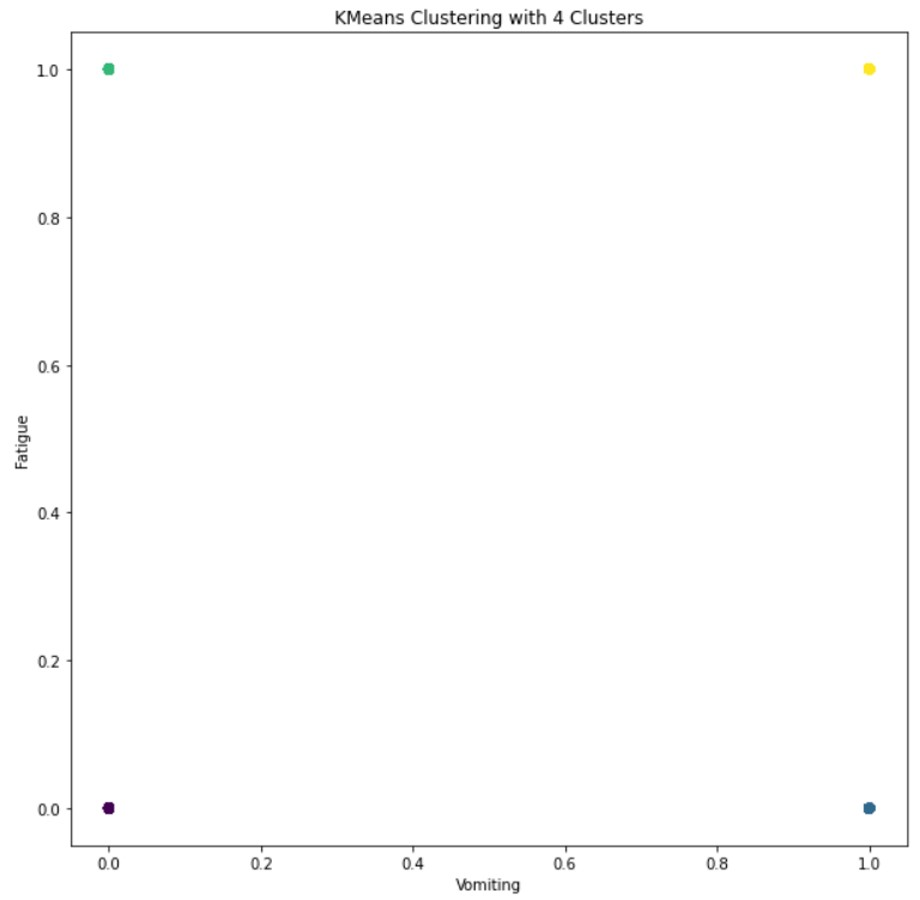
\includegraphics[scale=0.35]{j11}

\section*{Selección número de clusters adecuado}
Por el método del codo se calcula la inercia para entender que sucedería con la dispersión de los datos considerando 2 a 8 clusters.


\begin{tabular}{rrr} 
& nclusters & inertia \\
\hline $\mathbf{0}$ & 2 & $584.658$ \\
1 & 3 & $152.878$ \\
2 & 4 & $0.000$ \\
3 & 5 & $0.000$ \\
4 & 6 & $0.000$ \\
5 & 7 & $0.000$ \\
6 & 8 & $0.000$
\end{tabular}

Dada la información es binaria se sabe que debería ser suficiente con 4, pero se quiere entender como cambiaría añadiendo hasta 4 más, se espera que la diferencia sea pequeña o nula despues de cuatro. Además, se espera que sea muy grande menos de 4. 

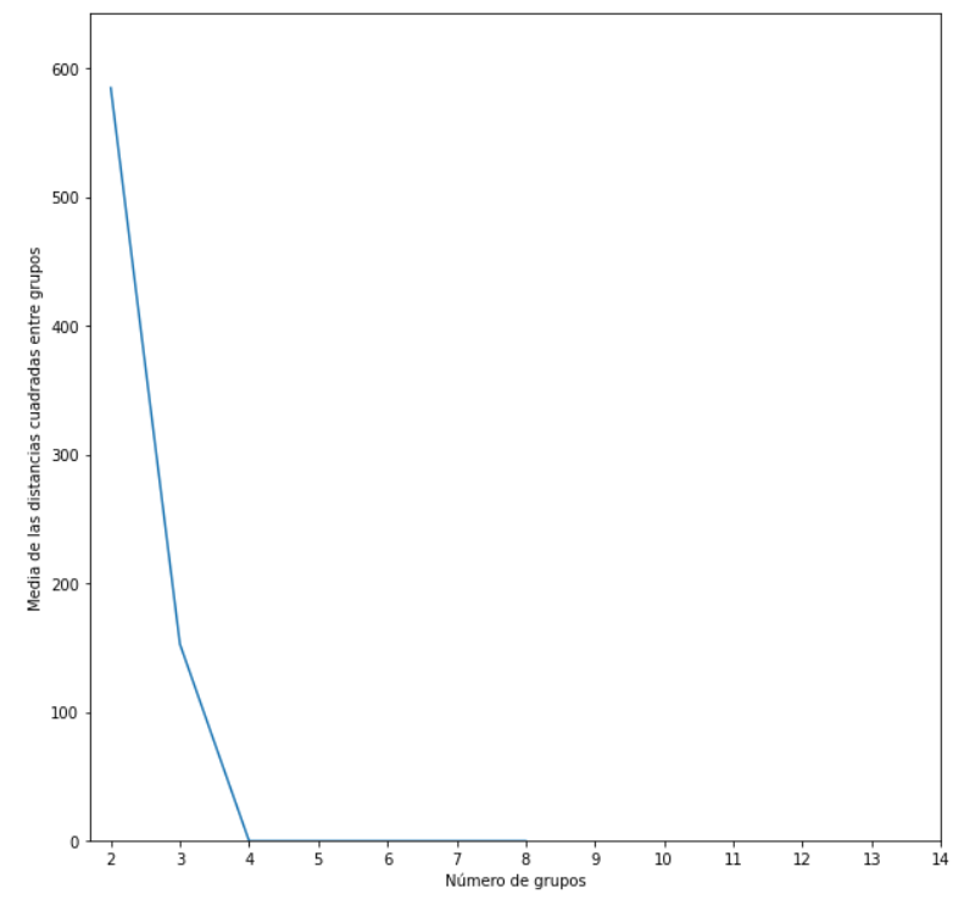
\includegraphics[scale=0.35]{j2}



\section*{Conclusion}
Lorem ipsum dolor sit amet, consectetur adipiscing elit, sed do eiusmod tempor incididunt ut labore et dolore magna aliqua. Massa tempor nec feugiat nisl pretium fusce id. Lorem sed risus ultricies tristique nulla. Nibh tortor id aliquet lectus proin nibh nisl condimentum id. Ornare arcu dui vivamus arcu felis bibendum ut tristique et. Scelerisque viverra mauris in aliquam sem fringilla ut. Molestie at elementum eu facilisis sed. Diam ut venenatis tellus in metus vulputate eu. Nibh venenatis cras sed felis eget velit aliquet. Egestas tellus rutrum tellus pellentesque eu tincidunt tortor. Nunc sed id semper risus in. Non tellus orci ac auctor augue mauris augue neque gravida. Libero enim sed faucibus turpis in eu mi bibendum neque. Id ornare arcu odio ut sem nulla pharetra. Ultrices tincidunt arcu non sodales neque sodales ut etiam.

\section*{List of abbreviations}
If abbreviations are used in the text they should be defined in the text at first use, and a list of abbreviations should be provided.







%%%%%%%%%%%%%%%%%%%%%%%%%%%%%%%%%%%%%%%%%%%%%%
%%                                          %%
%% Backmatter begins here                   %%
%%                                          %%
%%%%%%%%%%%%%%%%%%%%%%%%%%%%%%%%%%%%%%%%%%%%%%

\begin{backmatter}

\section*{Declarations}

\subsection*{Availability of data and materials}
The datasets used and/or analysed during the current study are available from the corresponding author on reasonable request.

\section*{Competing interests}
  The authors declare that they have no competing interests.

\section*{Author's contributions}
JRR was a major contributor in writing the manuscript.

\section*{Acknowledgements}
Universidad Autónoma de Nuevo León

\subsection*{Availability of data and materials}
The datasets used and/or analysed during the current study are available from the corresponding author on reasonable request.

\section*{Competing interests}
  The authors declare that they have no competing interests.

%%%%%%%%%%%%%%%%%%%%%%%%%%%%%%%%%%%%%%%%%%%%%%%%%%%%%%%%%%%%%
%%                  The Bibliography                       %%
%%                                                         %%
%%  Bmc_mathpys.bst  will be used to                       %%
%%  create a .BBL file for submission.                     %%
%%  After submission of the .TEX file,                     %%
%%  you will be prompted to submit your .BBL file.         %%
%%                                                         %%
%%                                                         %%
%%  Note that the displayed Bibliography will not          %%
%%  necessarily be rendered by Latex exactly as specified  %%
%%  in the online Instructions for Authors.                %%
%%                                                         %%
%%%%%%%%%%%%%%%%%%%%%%%%%%%%%%%%%%%%%%%%%%%%%%%%%%%%%%%%%%%%%

% if your bibliography is in bibtex format, use those commands:
\bibliographystyle{bmc-mathphys} % Style BST file (bmc-mathphys, vancouver, spbasic).
\bibliography{bmc_article}      % Bibliography file (usually '*.bib' )
% for author-year bibliography (bmc-mathphys or spbasic)
% a) write to bib file (bmc-mathphys only)
 %@settings{label, options="nameyear"}
% b) uncomment next line
%\nocite{label}

% or include bibliography directly:
%\begin{thebibliography}

%&\end{thebibliography}

%%%%%%%%%%%%%%%%%%%%%%%%%%%%%%%%%%%
%%                               %%
%% Figures                       %%
%%                               %%
%% NB: this is for captions and  %%
%% Titles. All graphics must be  %%
%% submitted separately and NOT  %%
%% included in the Tex document  %%
%%                               %%
%%%%%%%%%%%%%%%%%%%%%%%%%%%%%%%%%%%

%%
%% Do not use \listoffigures as most will included as separate files

\section*{Figures}
  \begin{figure}[h!]


  \caption{\csentence{Sample figure title.}
      A short description of the figure content
      should go here.}
      \end{figure}

\begin{figure}[h!]
  \caption{\csentence{Sample figure title.}
      Figure legend text.}
      \end{figure}

%%%%%%%%%%%%%%%%%%%%%%%%%%%%%%%%%%%
%%                               %%
%% Tables                        %%
%%                               %%
%%%%%%%%%%%%%%%%%%%%%%%%%%%%%%%%%%%

%% Use of \listoftables is discouraged.
%%
\section*{Tables}
\begin{table}[h!]
\caption{Sample table title. This is where the description of the table should go.}
      \begin{tabular}{cccc}
        \hline
           & B1  &B2   & B3\\ \hline
        A1 & 0.1 & 0.2 & 0.3\\
        A2 & ... & ..  & .\\
        A3 & ..  & .   & .\\ \hline
      \end{tabular}
\end{table}

%%%%%%%%%%%%%%%%%%%%%%%%%%%%%%%%%%%
%%                               %%
%% Additional Files              %%
%%                               %%
%%%%%%%%%%%%%%%%%%%%%%%%%%%%%%%%%%%

\section*{Additional Files}
  \subsection*{Additional file 1 --- Sample additional file title}
    Additional file descriptions text (including details of how to
    view the file, if it is in a non-standard format or the file extension).  This might
    refer to a multi-page table or a figure.

  \subsection*{Additional file 2 --- Sample additional file title}
    Additional file descriptions text.


\end{backmatter}
\end{document}
